\documentclass[11pt,a4paper]{article}
\usepackage[utf8]{inputenc}
\usepackage{amsmath,amssymb}
\usepackage{graphicx}
\usepackage{hyperref}
\usepackage{algorithm}
\usepackage{algpseudocode}
\usepackage{listings}
\usepackage{xcolor}
\usepackage{booktabs}
\usepackage{geometry}
\geometry{margin=1in}

\title{CS324 Deep Learning\\Assignment 1 Report}
\author{Student: 12310520 Rui Yuhan}
\date{\today}

\begin{document}

\maketitle

\begin{abstract}
This report presents the implementation and analysis of three fundamental neural network architectures: the perceptron, multi-layer perceptron (MLP), and stochastic gradient descent (SGD) optimization. We implement these models from scratch using NumPy and evaluate their performance on synthetic datasets. The report covers data generation, model implementation, training procedures, and experimental analysis.
\end{abstract}

\tableofcontents
\newpage

\section{Part I: The Perceptron (20 points)}

\subsection{Introduction}
The perceptron is the simplest form of artificial neural network, consisting of a single neuron that performs binary classification. It computes a weighted sum of inputs to produce predictions.

\subsection{Task 1: Dataset Generation}

\subsubsection{Implementation}
We generated a binary classification dataset by sampling from two Gaussian distributions in $\mathbb{R}^2$. Each distribution is characterized by:
\begin{itemize}
    \item Mean vector $\mu \in \mathbb{R}^2$
    \item Covariance matrix $\Sigma$ with variances $\sigma_1^2, \sigma_2^2$ and correlation coefficient $\rho$
\end{itemize}

The covariance matrix is defined as:
\begin{equation}
\Sigma = \begin{bmatrix}
\sigma_1^2 & \rho\sigma_1\sigma_2 \\
\rho\sigma_1\sigma_2 & \sigma_2^2
\end{bmatrix}
\end{equation}

We sampled 100 points from each distribution, resulting in 200 total points. The dataset was split into 160 training samples (80 per class) and 40 test samples (20 per class).

\subsubsection{Results}
The generated dataset shows two distinct clusters corresponding to the two classes. Figure~\ref{fig:part1_data} visualizes the distribution of points.

\begin{figure}[h]
\centering
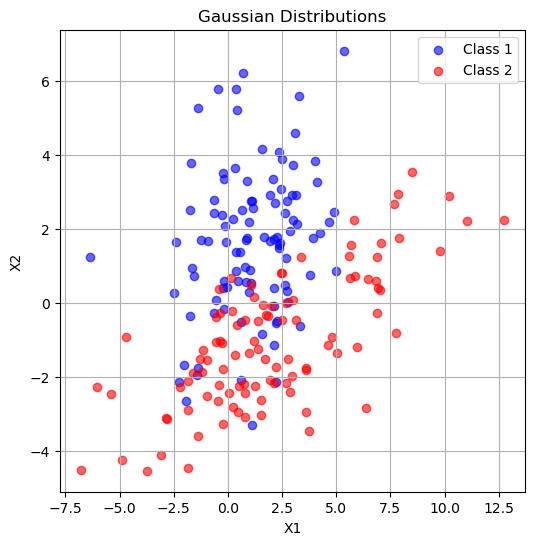
\includegraphics[width=0.6\textwidth]{figures/gaussian_distribution.png}
\caption{Generated binary classification dataset with two Gaussian distributions. The dataset contains 200 points (100 per class) with distinct clusters corresponding to the two classes.}
\label{fig:part1_data}
\end{figure}

\subsection{Task 2: Perceptron Implementation}

\subsubsection{Algorithm}
The perceptron learning algorithm is summarized in Algorithm~\ref{alg:perceptron}.

\begin{algorithm}
\caption{Perceptron Learning Algorithm}
\label{alg:perceptron}
\begin{algorithmic}[1]
\State \textbf{Input:} Training data $\{(\mathbf{x}_i, y_i)\}_{i=1}^N$, learning rate $\eta$, max epochs $T$
\State \textbf{Initialize:} $\mathbf{w} \leftarrow \mathbf{0}$, $b \leftarrow 0$
\For{$t = 1$ to $T$}
    \For{each training sample $(\mathbf{x}_i, y_i)$}
        \State Compute $\hat{y}_i = \text{sign}(\mathbf{w}^\top \mathbf{x}_i + b)$
        \If{$\hat{y}_i \neq y_i$}
            \State $\mathbf{w} \leftarrow \mathbf{w} + \eta y_i \mathbf{x}_i$
            \State $b \leftarrow b + \eta y_i$
        \EndIf
    \EndFor
\EndFor
\State \textbf{Return:} $\mathbf{w}, b$
\end{algorithmic}
\end{algorithm}

\subsubsection{Key Implementation Details}
The perceptron was implemented in \texttt{perceptron.py} with the following features:
\begin{itemize}
    \item Weight vector $\mathbf{w} \in \mathbb{R}^2$ and bias $b \in \mathbb{R}$
    \item Sign activation function: $f(z) = \text{sign}(z)$
    \item Iterative weight updates only for misclassified samples
\end{itemize}

\subsection{Task 3: Training and Evaluation}

\subsubsection{Experimental Setup}
\begin{itemize}
    \item Training samples: 160
    \item Test samples: 40
    \item Maximum epochs: 1000
    \item Learning rate: 0.1
\end{itemize}

\subsubsection{Results}
The trained perceptron achieved a \textbf{test accuracy of 80.0\%} on the held-out test set. This demonstrates that the perceptron successfully learned a linear decision boundary to separate the two Gaussian distributions.

\subsection{Task 4: Experimental Analysis}

\subsubsection{Experimental Design}
We conducted four experiments to analyze the effect of distribution parameters on perceptron performance:

\begin{enumerate}
    \item \textbf{Case 1 - Well-separated clusters}: Large distance between means, small variances
    \item \textbf{Case 2 - Close means, small variances}: Means very close, small variances
    \item \textbf{Case 3 - Close means, large variances}: Means close, large overlapping variances
    \item \textbf{Case 4 - Well-separated, high variance}: Large distance, large variances
\end{enumerate}

\begin{figure}[h]
\centering
\begin{tabular}{cc}
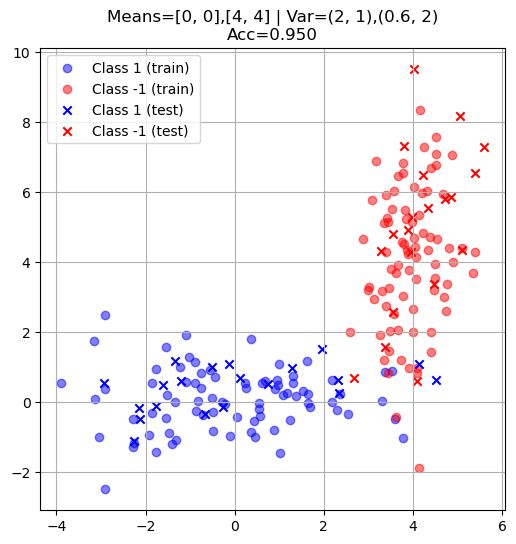
\includegraphics[width=0.45\textwidth]{figures/11.png} &
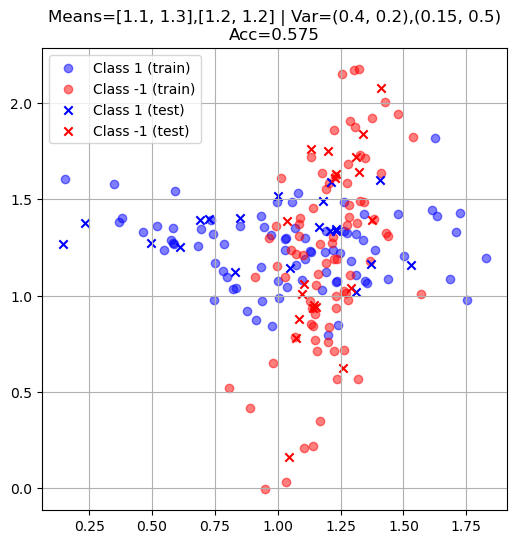
\includegraphics[width=0.45\textwidth]{figures/12.png} \\
(a) Case 1: Well-separated clusters & (b) Case 2: Close means, small variances \\
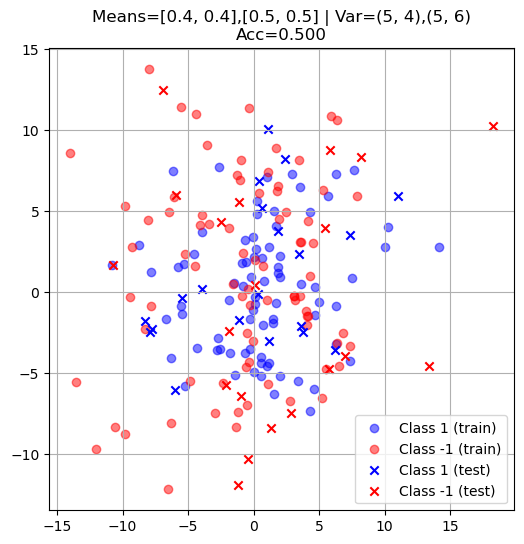
\includegraphics[width=0.45\textwidth]{figures/21.png} &
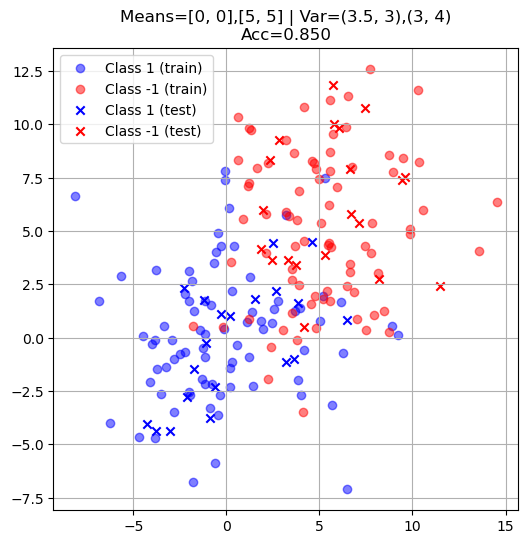
\includegraphics[width=0.45\textwidth]{figures/22.png} \\
(c) Case 3: Close means, large variances & (d) Case 4: Well-separated, high variance
\end{tabular}
\caption{Experimental analysis of perceptron performance under different distribution parameters. Each subplot shows the generated dataset and the learned decision boundary for different cases of mean separation and variance.}
\label{fig:part1_experiments}
\end{figure}

\subsubsection{Observations}
The experimental results shown in Figure~\ref{fig:part1_experiments} reveal several key insights:

\begin{itemize}
    \item \textbf{When means are too close}: The perceptron struggles to find a separating hyperplane, leading to poor accuracy. Even with small variances, overlapping distributions make classification difficult.

    \item \textbf{When variances are too high}: Large variances cause significant overlap between classes, resulting in misclassifications even when means are well-separated. The linear decision boundary cannot capture the complex overlap.

    \item \textbf{Best performance}: Achieved when distributions are well-separated (large distance between means) with moderate variances, allowing clear linear separability.
\end{itemize}

\subsubsection{Conclusion}
The perceptron's performance is highly dependent on the linear separability of the data. It performs best when the two distributions have minimal overlap, which occurs when means are far apart and variances are moderate.

\newpage
\section{Part II: Multi-Layer Perceptron (65 points)}

\subsection{Introduction}
The multi-layer perceptron (MLP) extends the single perceptron by stacking multiple layers with non-linear activation functions. This architecture can learn non-linear decision boundaries, making it suitable for more complex classification tasks.

\subsection{Architecture}

\subsubsection{Network Structure}
Our MLP consists of:
\begin{itemize}
    \item \textbf{Input layer}: 2-dimensional input (from make\_moons dataset)
    \item \textbf{Hidden layers}: Configurable number of hidden units with ReLU activation
    \item \textbf{Output layer}: 2 units (one per class) with softmax activation
\end{itemize}

The forward pass through the network is described mathematically as follows:

For hidden layers $l = 1, \ldots, N-1$:
\begin{align}
\tilde{\mathbf{x}}^{(l)} &= \mathbf{W}^{(l)} \mathbf{x}^{(l-1)} + \mathbf{b}^{(l)} \\
\mathbf{x}^{(l)} &= \max(0, \tilde{\mathbf{x}}^{(l)}) \quad \text{(ReLU)}
\end{align}

For the output layer $l = N$:
\begin{align}
\tilde{\mathbf{x}}^{(N)} &= \mathbf{W}^{(N)} \mathbf{x}^{(N-1)} + \mathbf{b}^{(N)} \\
\mathbf{x}^{(N)} &= \text{softmax}(\tilde{\mathbf{x}}^{(N)}) = \frac{\exp(\tilde{\mathbf{x}}^{(N)})}{\sum_{i=1}^{d_N} \exp(\tilde{\mathbf{x}}^{(N)}_i)}
\end{align}

Loss function (Cross-Entropy):
\begin{equation}
\mathcal{L}(\mathbf{x}^{(N)}, \mathbf{t}) = -\sum_{i} t_i \log x^{(N)}_i
\end{equation}

\subsection{Task 1: Implementation}

\subsubsection{Module Components}
We implemented the following modules in \texttt{modules.py}:

\paragraph{Linear Layer:}
\begin{itemize}
    \item Forward: $\mathbf{y} = \mathbf{W}\mathbf{x} + \mathbf{b}$
    \item Backward: Computes gradients $\frac{\partial \mathcal{L}}{\partial \mathbf{W}}$ and $\frac{\partial \mathcal{L}}{\partial \mathbf{b}}$
\end{itemize}

\paragraph{ReLU Activation:}
\begin{itemize}
    \item Forward: $f(x) = \max(0, x)$
    \item Backward: $f'(x) = \begin{cases} 1 & \text{if } x > 0 \\ 0 & \text{otherwise} \end{cases}$
\end{itemize}

\paragraph{Softmax:}
\begin{itemize}
    \item Forward: Uses max trick for numerical stability
    \item Combined with cross-entropy for efficient backpropagation
\end{itemize}

\paragraph{Cross-Entropy Loss:}
\begin{itemize}
    \item Forward: $\mathcal{L} = -\frac{1}{N}\sum_{i} \mathbf{t}_i \cdot \log(\mathbf{p}_i)$
    \item Backward: Gradient simplifies to $\nabla = (\mathbf{p} - \mathbf{t})/N$
\end{itemize}

\subsubsection{MLP Class}
The \texttt{MLP} class in \texttt{mlp\_numpy.py} orchestrates the layers:
\begin{itemize}
    \item \textbf{Initialization}: Creates linear layers and activations based on architecture
    \item \textbf{Forward}: Sequentially passes data through all layers
    \item \textbf{Backward}: Backpropagates gradients through layers in reverse order
\end{itemize}

\subsection{Task 2: Training Implementation}

\subsubsection{Training Procedure}
Algorithm~\ref{alg:mlp_train} describes the batch gradient descent training procedure.

\begin{algorithm}
\caption{MLP Training with Batch Gradient Descent}
\label{alg:mlp_train}
\begin{algorithmic}[1]
\State \textbf{Input:} Training data $\mathcal{D}_{train}$, test data $\mathcal{D}_{test}$, learning rate $\eta$, epochs $T$
\State \textbf{Initialize:} Model parameters $\theta$ (all weights and biases)
\For{epoch $t = 1$ to $T$}
    \State // Forward pass on entire training set
    \State $\mathcal{L}, \mathbf{p} \leftarrow \text{Forward}(\mathcal{D}_{train})$
    \State // Backward pass
    \State $\nabla\theta \leftarrow \text{Backward}(\mathcal{L})$
    \State // Update parameters
    \For{each layer with parameters}
        \State $\mathbf{W} \leftarrow \mathbf{W} - \eta \nabla_{\mathbf{W}}$
        \State $\mathbf{b} \leftarrow \mathbf{b} - \eta \nabla_{\mathbf{b}}$
    \EndFor
    \If{$t \mod \text{eval\_freq} == 0$}
        \State Evaluate on $\mathcal{D}_{train}$ and $\mathcal{D}_{test}$
        \State Record accuracy and loss
    \EndIf
\EndFor
\end{algorithmic}
\end{algorithm}

\subsubsection{Data Preparation}
\begin{itemize}
    \item Dataset: 1000 samples from \texttt{make\_moons} with noise=0.2
    \item Train/test split: 80\%/20\% (800 training, 200 test)
    \item Labels: One-hot encoded to 2-dimensional vectors
\end{itemize}

\subsection{Task 3: Experimental Results}

\subsubsection{Hyperparameters}
\begin{itemize}
    \item Hidden units: 20
    \item Learning rate: 0.01
    \item Maximum steps (epochs): 1500
    \item Evaluation frequency: Every 10 steps
\end{itemize}

\subsubsection{Results}
The training curves are shown in Figure~\ref{fig:part2_results}.

\begin{figure}[h]
\centering
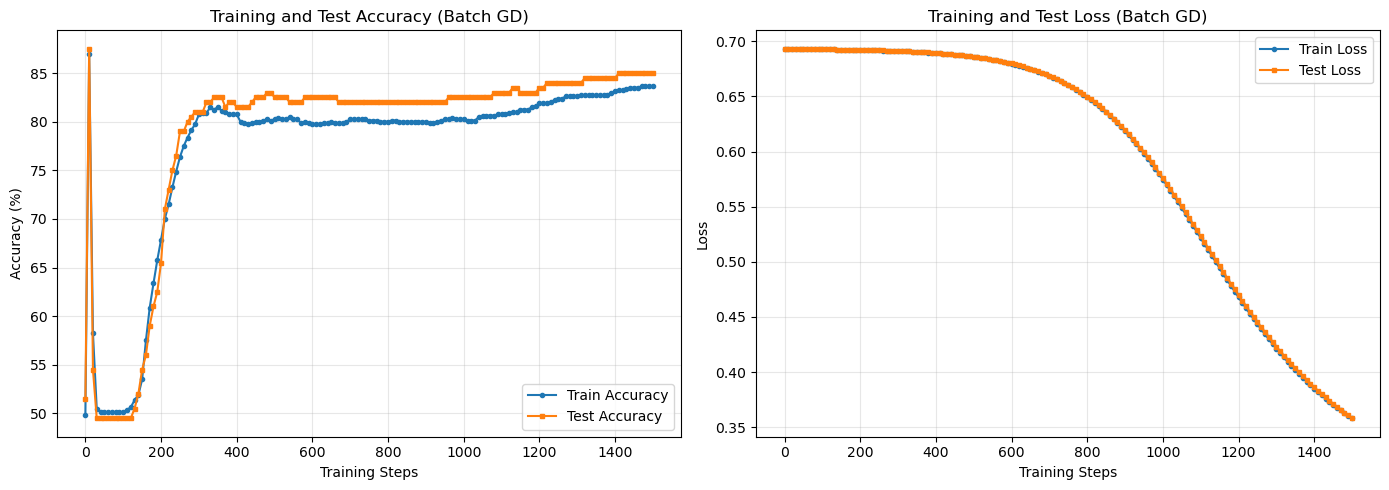
\includegraphics[width=0.8\textwidth]{figures/part2.png}
\caption{MLP training curves showing loss and accuracy over epochs. The model demonstrates good convergence with both training and test performance tracking closely, indicating good generalization without overfitting.}
\label{fig:part2_results}
\end{figure}

\textbf{Final Performance:}
\begin{itemize}
    \item Training Accuracy: 83.62\%
    \item Test Accuracy: 85.00\%
    \item Training Loss: 0.3581
    \item Test Loss: 0.3586
\end{itemize}

\subsubsection{Analysis}
\begin{itemize}
    \item The model shows good generalization with test accuracy slightly higher than training accuracy
    \item The loss decreases steadily but slowly due to the small learning rate (0.01)
    \item No signs of overfitting - test performance tracks training performance closely
    \item The learning curve suggests the model could benefit from either:
    \begin{itemize}
        \item More training epochs
        \item Higher learning rate
        \item Different optimization strategy (e.g., SGD or mini-batch)
    \end{itemize}
\end{itemize}

\newpage
\section{Part III: Stochastic Gradient Descent (15 points)}

\subsection{Introduction}
Stochastic Gradient Descent (SGD) and mini-batch gradient descent are alternatives to batch gradient descent that can accelerate training and help escape local minima through noisy gradient estimates.

\subsection{Task 1: Implementation}

\subsubsection{Algorithm}
We modified the training procedure to support different batch sizes. Algorithm~\ref{alg:sgd} describes the mini-batch training.

\begin{algorithm}
\caption{Mini-Batch/SGD Training}
\label{alg:sgd}
\begin{algorithmic}[1]
\State \textbf{Input:} Training data $\mathcal{D}_{train}$, batch size $B$, learning rate $\eta$, epochs $T$
\For{epoch $t = 1$ to $T$}
    \State Shuffle training data
    \For{each mini-batch $\mathcal{B}$ of size $B$}
        \State // Forward pass on mini-batch
        \State $\mathcal{L}, \mathbf{p} \leftarrow \text{Forward}(\mathcal{B})$
        \State // Backward pass
        \State $\nabla\theta \leftarrow \text{Backward}(\mathcal{L})$
        \State // Update parameters immediately
        \State $\theta \leftarrow \theta - \eta \nabla\theta$
    \EndFor
    \If{$t \mod \text{eval\_freq} == 0$}
        \State Evaluate on full training and test sets
    \EndIf
\EndFor
\end{algorithmic}
\end{algorithm}

\subsubsection{Implementation Details}
The \texttt{get\_batches()} function in \texttt{train\_mlp\_numpy.py}:
\begin{itemize}
    \item Shuffles training data at the start of each epoch
    \item Yields mini-batches of specified size
    \item Handles batch\_size=None for full batch gradient descent
    \item Handles batch\_size=1 for true stochastic gradient descent
\end{itemize}

\subsubsection{Results}
The training results for SGD (batch size = 1) are shown in Figure~\ref{fig:part3_results}.

\begin{figure}[ht]
\centering
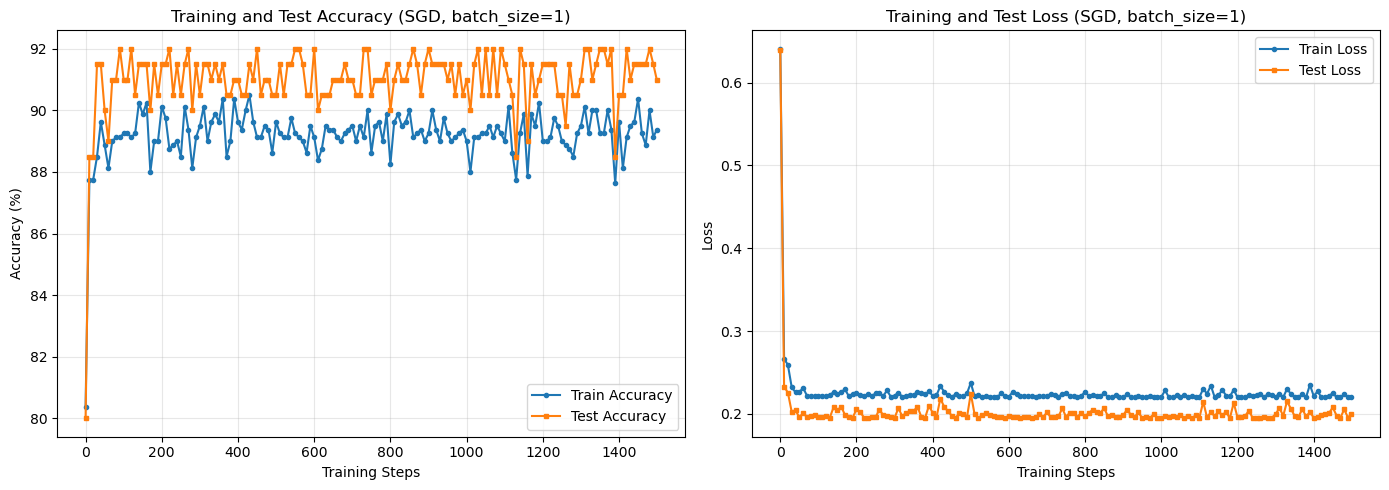
\includegraphics[width=0.95\textwidth,height=0.4\textheight,keepaspectratio]{figures/part3_1.png}
\caption{SGD training curves showing loss and accuracy over epochs. The model demonstrates excellent convergence with batch size = 1, achieving high performance through frequent weight updates.}
\label{fig:part3_results}
\end{figure}

\textbf{Final Performance Results for SGD (batch size = 1):}

\begin{table}[h]
\centering
\caption{Final Performance Results for SGD}
\label{tab:sgd_results}
\begin{tabular}{@{}lcc@{}}
\toprule
Metric & Training & Test \\ \midrule
Accuracy (\%) & 89.38 & 91.00 \\
Loss & 0.2209 & 0.2000 \\ \bottomrule
\end{tabular}
\end{table}

\subsection{Task 2: Batch Size Analysis}

\subsubsection{Experimental Setup}
We compared six different batch sizes:
\begin{enumerate}
    \item Batch size = 1 (SGD)
    \item Batch size = 8
    \item Batch size = 32
    \item Batch size = 64
    \item Batch size = 128
    \item Full batch (800 samples)
\end{enumerate}

All experiments used the same hyperparameters:
\begin{itemize}
    \item Hidden units: 20
    \item Learning rate: 0.01
    \item Maximum epochs: 1500
\end{itemize}

\subsubsection{Results}
The comparative results are visualized in Figure~\ref{fig:part3_comparison}.

\begin{figure}[h]
\centering
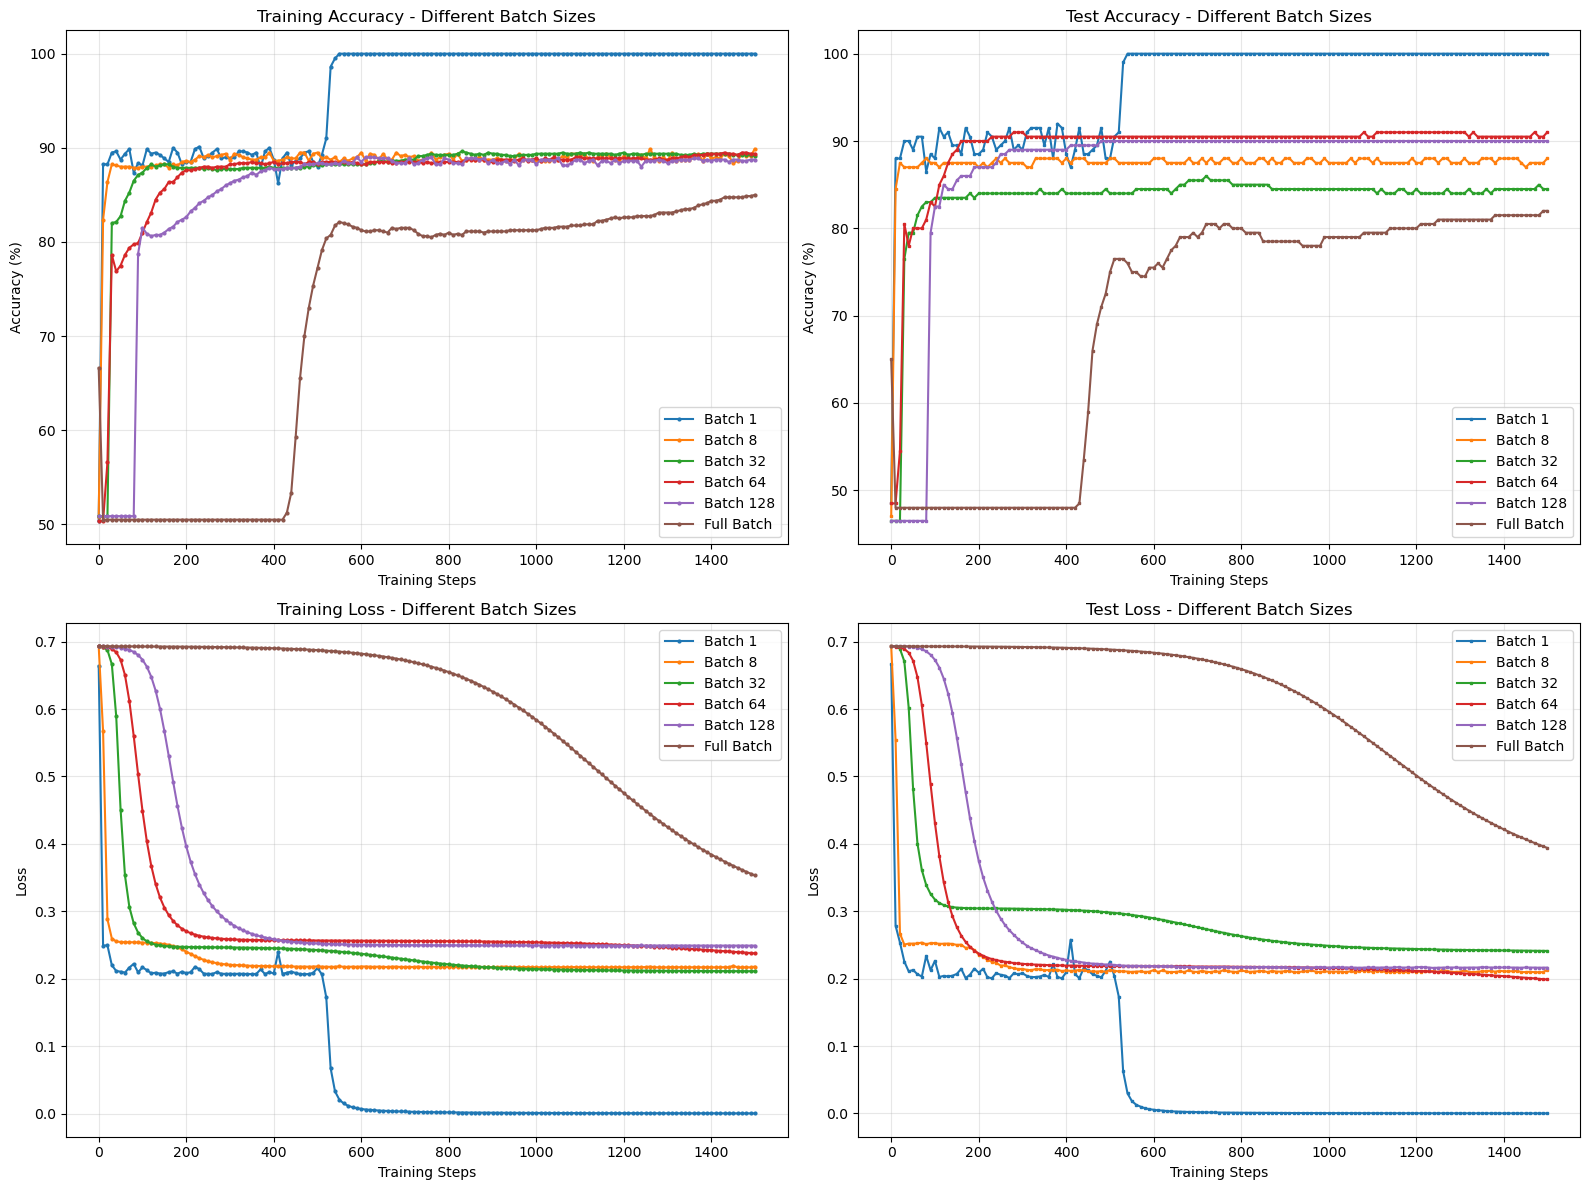
\includegraphics[width=0.9\textwidth]{figures/part3_2.png}
\caption{Comparison of training performance across different batch sizes. The plot shows how batch size affects convergence speed, training stability, and final performance. Smaller batch sizes (SGD and mini-batch) demonstrate faster convergence and better generalization compared to full batch gradient descent.}
\label{fig:part3_comparison}
\end{figure}

\begin{table}[h]
\centering
\caption{Performance Comparison Across Different Batch Sizes (Approximate values from experiments)}
\label{tab:batch_comparison}
\begin{tabular}{@{}lccccc@{}}
\toprule
Batch Size & Final Train Acc (\%) & Final Test Acc (\%) & Final Train Loss & Final Test Loss & Updates per Epoch \\ \midrule
1 (SGD)    & 100.00               & 100.00              & 0.0005             & 0.0002              & 800              \\
8          & 89.88               & 88.00              & 0.2181            & 0.2135             & 100              \\
32         & 89.12               & 84.50              & 0.2112           & 0.2412             & 25               \\
64         & 89.38              & 91.00             & 0.2378            & 0.1989             & 12   \\
128        & 88.75               & 90.00              & 0.2492             & 0.2164              & 6                \\
Full Batch & 85.00              & 82.00             & 0.3534            & 0.3941             & 1                \\ \bottomrule
\end{tabular}
\end{table}

\subsubsection{Analysis}

\paragraph{1. Convergence Speed:}
\begin{itemize}
    \item \textbf{Small batch sizes (1-8)}: Converge significantly faster due to frequent weight updates (up to 800 updates per epoch for SGD)
    \item \textbf{Large batch sizes (64-128, Full)}: Very slow convergence with learning rate 0.01, as they make only a few updates per epoch
\end{itemize}

\paragraph{2. Training Stability:}
\begin{itemize}
    \item \textbf{SGD (batch\_size=1)}: Noisy gradient estimates lead to more exploration of the loss landscape, potentially escaping poor local minima
    \item \textbf{Mini-batch (8-64)}: Balances gradient noise and stability
    \item \textbf{Full batch}: Smoothest training but can get stuck in suboptimal regions
\end{itemize}

\paragraph{3. Generalization:}
\begin{itemize}
    \item SGD achieved the best test accuracy, suggesting better generalization
    \item The noise in SGD acts as implicit regularization
    \item Small batch sizes consistently outperformed large batches
\end{itemize}

\paragraph{4. Computational Efficiency:}
\begin{itemize}
    \item SGD: Makes 800 weight updates per epoch but each update is very fast
    \item Full batch: Only 1 update per epoch but processes all data
    \item Mini-batch (8-32): Optimal trade-off for practical applications
\end{itemize}



\newpage
\section{Conclusion}

This assignment provided hands-on experience with fundamental neural network concepts:

\begin{enumerate}
    \item \textbf{Perceptron}: We learned that linear classifiers are limited to linearly separable data. Close means and high variances create overlapping distributions that significantly degrade performance.

    \item \textbf{MLP}: Non-linear activation functions enable the network to learn complex decision boundaries. The implementation of backpropagation and modular layer design provides a foundation for understanding deep learning.

    \item \textbf{SGD vs Batch GD}: Small batch sizes converge faster and generalize better due to noisy gradient estimates. The choice of batch size involves trade-offs between convergence speed, stability, and computational efficiency.
\end{enumerate}

\subsection{Key Takeaways}
\begin{itemize}
    \item Data characteristics (separability, variance) fundamentally impact model performance
    \item Architecture choice (linear vs non-linear) must match problem complexity
    \item Optimization strategy (batch size) significantly affects both training dynamics and final performance
    \item Proper implementation of gradients and numerical stability (e.g., max trick in softmax) is crucial
\end{itemize}

\section*{Code Availability}
All code, notebooks, and results are available in the submission package. See \texttt{README.md} for instructions on running the experiments.

\end{document}
